%=== Einheit  ====================================================================
\Tut\chapter{Regul\"are Ausdr\"ucke und rechtslineare Grammatiken}
\label{k:reg-ausdruecke}

Am Ende von \hyperref[k:endl-auto]{Einheit~\ref{k:endl-auto} über
  endliche Automaten} haben wir gesehen, dass manche formale Sprachen
zwar von kontextfreien Grammatiken erzeugt, aber nicht von endlichen
Akzeptoren erkannt werden können. Damit stellt sich für Sie vielleicht
zum ersten Mal die Frage nach einer \emph{Charakterisierung}, nämlich
der der mit endlichen Akzeptoren erkennbaren Sprachen. Damit ist eine
präzise Beschreibung dieser formalen Sprachen gemeint, die nicht (oder
jedenfalls nicht offensichtlich) Automaten benutzt.

In den beiden Abschnitten dieser Einheit werden Sie zwei solche
Charakterisierungen kennenlernen, die über
\hyperref[sec:reg-ausdruecke]{reguläre Ausdrücke} und die über
\hyperref[sec:rechtslineare-grammatiken]{rechtslineare
  Grammatiken}. In Abschnitt~\ref{sec:strukturelle-induktion} wird es
unter anderem um eine bequeme Verallgemeinerung vollständiger
Induktion gehen.

%-----------------------------------------------------------------------
\Tut\section{Regul\"are Ausdr\"ucke}
\label{sec:reg-ausdruecke}

Der Begriff \emph{regulärer Ausdruck} geht ursprünglich auf Stephen
\textcite{Kleene_1956_REN_ic}\index{Kleene, Stephen Cole} zurück und
wird heute in unterschiedlichen Bedeutungen genutzt.  In dieser
Einheit führen wir kurz regulären Ausdrücken nach der "`klassischen"'
Definition ein.

Etwas anderes (nämlich allgemeineres) sind die Varianten der
\emph{Regular Expressions}, von denen Sie möglicherweise schon im
Zusammenhang mit dem ein oder anderen Programm (emacs, grep, sed,
\dots) oder der ein oder anderen Programmiersprache (Java, Python,
\dots) gelesen haben. Für Java gibt es das Paket
\href{http://java.sun.com/javase/6/docs/api/java/util/regex/package-summary.html}{java.util.regex}.
Regular expressions sind eine deutliche Verallgemeinerung regulärer
Ausdrücke, auf die wir in dieser Vorlesung nicht eingehen werden.
Alles was wir im folgenden über reguläre Ausdrücke sagen, ist aber
auch bei regular expressions anwendbar.

Wir kommen direkt zur Definition regulärer Ausdrücke. Sie wird sie
hoffentlich an das ein oder andere aus der
\hyperref[k:sprachen]{Einheit~\ref{k:sprachen} über formale Sprachen}
und die zugehörigen Übungsaufgaben erinnern.

Es sei $A$ ein Alphabet, das keines der fünf Zeichen aus $Z=\{\rx|,
\rx(, \rx), \rx*, \rx{O}\}$ enthält.  Ein \mdefine{regulärer
  Ausdruck}\index{regulärer Ausdruck} über $A$ ist eine Zeichenfolge
über dem Alphabet $A\cup Z$, die gewissen Vorschriften genügt. Die
Menge der regulären Ausdrücke ist wie folgt festgelegt:
% 
\begin{itemize}
\item $\rx{O}$ ist ein regulärer Ausdruck.
\item Für jedes $x\in A$ ist $x$ ein regulärer Ausdruck.
\item Wenn $R_1$ und $R_2$ reguläre Ausdrücke sind, dann sind auch
  $\rx(R_1 \rx| R_2\rx)$ und $\rx(R_1R_2\rx)$ reguläre Ausdrücke.
\item Wenn $R$ ein regulärer Ausdruck ist, dann auch $\rx(R\rx*\rx)$.
\item Nichts anderes sind reguläre Ausdrücke.
\end{itemize}
% 
Um sich das Schreiben zu vereinfachen, darf man Klammern auch
weglassen. Im Zweifelsfall gilt "`Stern- vor Punkt- und Punkt- vor
Strichrechnung"', \dh $R_1 \rx| R_2R_3\rx*$ ist \zB als $\rx(R_1
\rx| \rx(R_2\rx(R_3\rx*\rx)\rx)\rx)$ zu verstehen. Bei mehreren
gleichen binären Operatoren gilt das als links geklammert; zum
Beispiel ist $R_1 \rx| R_2 \rx| R_3$ als $\rx( \rx(R_1 \rx| R_2\rx)
\rx| R_3 \rx)$ zu verstehen.

\begin{tutorium}
  \subsubsection*{Klammereinsparungsregeln}
  \begin{itemize}
  \item sind wohl sinnvoll und naheliegend gewählt
  \item muss man daher hoffentlich nicht groß auswendig lernen
  \item zumal es dann für $\lang{R}$ sowieso egal ist, ob man von
    links oder von rechts klammert: \zB
    $\lang{\rx{((aa)b)}}=\lang{\rx{(a(ab))}} = \{\#{aab}\}$
  \item aber sind $\rx{((aa)b)}$ und $\rx{(a(ab))}$ verschiedene
    reguläre Ausdrücke (wenn sie auch die gleiche formale Sprache
    beschreiben)
  \end{itemize}
\end{tutorium}

Man kann die korrekte Syntax regulärer Ausdrücke auch mit Hilfe einer
kontextfreien Grammatik beschreiben: Zu gegebenem Alphabet $A$ sind
die legalen regulären Ausdrücke gerade die Wörter, die von der
Grammatik
\begin{align*}
  G &= (\{R\}, \; \{\rx|, \rx(, \rx), \rx*, \rx{O}\}\cup A,\; R,\; P) \\
  \text{mit\quad } P &= \{ R-> \rx{O},\;\; R-> \rx( R\rx|R\rx),\;\; R-> \rx(RR\rx),\;\; R-> \rx(R\rx*\rx) \}\\
  &\quad\cup \{ R-> x \mid x\in A\} 
\end{align*}
erzeugt werden.

\begin{tutorium}
  \subsubsection*{kontextfreie Grammatik, die die regulären Ausdrücke erzeugt}
  \begin{itemize}
  \item habe lange überlegt, ob ich die mit rein nehme
  \item \textbf{Vorsicht Gefahr:} nicht durcheinander bringen. Die
    \emph{Syntax} regulärer Ausdrücke ist kontextfrei, aber die
    Bedeutung, \ie \emph{Semantik}, regulärer Ausdrücke sind nur
    reguläre Sprachen
  \item \textbf{aber auch lehrreich:} mal wieder Unterschied
    zwischen Syntax (Typ-2-Sprache) und Semantik (Typ-3-Sprachen)
  \end{itemize}
\end{tutorium}

Die folgenden Zeichenketten sind alle reguläre Ausdrücke über dem
Alphabet $\{\#a,\#b\}$:

   \begin{tabular}{>{\textbullet\hspace*{1ex}}p{20mm}>{\textbullet\hspace*{1ex}}p{20mm}>{\textbullet\hspace*{1ex}}p{29mm}>{\textbullet\hspace*{1ex}}p{28mm}}
     \rx O        & \rx{a}          & \multicolumn{2}{l}{\textbullet\hspace*{1ex} \rx{b}}              \\
     \rx{(ab)}    & \rx{((ab)a)}  & \rx{(((ab)a)a)}   & \rx{((ab)(aa))}   \\
     \rx{(O|b)}   & \rx{(a|b)}    & \rx{((a(a|b))|b)} & \rx{(a|(b|(a|a)))} \\
     \rx{(O*)}    & \rx{(a*)}     & \rx{((ba)(b*))}   & \rx{(((ba)b)*)}   \\
     \rx{((a*)*)} & \multicolumn{3}{l}{\textbullet\hspace*{1ex}\rx{(((((ab)b)*)*)|(O*))}}  \\
   \end{tabular} \\
% \begin{tabular}{*{4}{>{\makebox[6mm]{(\alph{thwmini})\quad}\incthwmini}p{30mm}}}
%      \rx O        & \rx{a}          & \multicolumn{2}{l}{\textbullet\hspace*{1ex} \rx{b}}              \\
%      \rx{(ab)}    & \rx{((ab)a)}  & \rx{(((ab)a)a)}   & \rx{((ab)(aa))}   \\
%      \rx{(O|b)}   & \rx{(a|b)}    & \rx{((a(a|b))|b)} & \rx{(a|(b|(a|a)))} \\
%      \rx{(O*)}    & \rx{(a*)}     & \rx{((ba)(b*))}   & \rx{(((ba)b)*)}   \\
%      \rx{((a*)*)} & \multicolumn{3}{l}{\textbullet\hspace*{1ex}\rx{(((((ab)b)*)*)|(O*))}}  \\
% \end{tabular}\\

\noindent
Wendet man die Klammereinsparungsregeln an, so ergibt sich aus
den Beispielen mit Klammern:\\
  \begin{tabular}{>{\textbullet\hspace*{1ex}}p{20mm}>{\textbullet\hspace*{1ex}}p{20mm}>{\textbullet\hspace*{1ex}}p{29mm}>{\textbullet\hspace*{1ex}}p{28mm}}
    \rx{ab}  & \rx{aba} & \rx{abaa}     & \rx{ab(aa) } \\
    \rx{O|b} & \rx{a|b} & \rx{a(a|b)|b} & \rx{(a|(b|(a|a)))} \\
    \rx{O*}  & \rx{a*}  & \rx{bab*}     & \rx{(bab)*} \\
    \rx{a**} & \multicolumn{3}{l}{\textbullet\hspace*{1ex}\rx{(abb)**|O*}} \\
  \end{tabular}\\
% \setcounter{thwmini}{4}
% \begin{tabular}{*{4}{>{\makebox[6mm]{(\alph{thwmini})\addtocounter{thwmini}{1}\quad}}p{30mm}}}
%   \rx{01}  & \rx{010} & \rx{0100}     \\
%   \rx{01(00)} & \rx{O|1} & \rx{0|1} \\
%   \rx{0(0|1)|1} & \rx{(0|(1|(0|0)))} & \rx{O*} \\
%   \rx{0*}  & \rx{101*}     & \rx{(101)*} \\
%   \rx{0**} & \rx{(011)**|O*} \\
% \end{tabular}\\

\noindent
Die folgenden Zeichenketten sind dagegen auch bei Berücksichtigung
der Klammereinsparungsregeln \emph{keine} regulären Ausdrücke über
$\{\#a,\#b\}$:

  \begin{tabular}{l@{\qquad }p{0.75\textwidth}}
    \rx{(|b)}  & vor \rx| fehlt ein regulärer Ausdruck  \\
    \rx{|O|}   & vor und hinter \rx| fehlt je ein regulärer Ausdruck \\
    \rx{()ab}  & zwischen \rx( und \rx) fehlt ein regulärer Ausdruck \\
    \rx{((ab)} & Klammern müssen "`gepaart"' auftreten \\
    \rx{*(ab)} & vor \rx* fehlt ein regulärer Ausdruck  \\
    \rx{c*}    & \leavevmode \rx{c} ist nicht Zeichen des Alphabetes \\
  \end{tabular}\\
% \begin{tabular}{l@{\ }>{falsch: }p{0.75\textwidth}<{;}}
%   \rx{(|1)}  & vor \rx| fehlt ein regulärer Ausdruck  \\
%   \rx{|O|}   & vor und hinter \rx| fehlt je ein regulärer Ausdruck \\
%   \rx{()01}  & zwischen \rx( und \rx) fehlt ein regulärer Ausdruck \\
%   \rx{((01)} & Klammern müssen "`in der üblichen Weise gepaart"' auftreten \\
%   \rx{*(01)} & vor \rx* fehlt ein regulärer Ausdruck  \\
%   \rx{2*}    & \rx2 ist nicht Zeichen des Alphabetes \\
% \end{tabular}\\

\noindent
Reguläre Ausdrücke werden benutzt, um formale Sprachen zu
spezifizieren. Auch dafür bedient man sich wieder einer induktiven
Vorgehensweise; man spricht auch von einer induktiven Definition:

Die \mdefine[durch $R$ beschriebene Sprache $\lang{R}$]{von einem
  regulären Ausdruck $R$ beschriebene formale Sprache}
$\lang{R}$\index{R@{$\lang{R}$}} ist wie folgt definiert:
% 
\begin{itemize}
\item $\lang{\rx{O}} = \{\}$ (\dh die leere Menge).
\item Für $x\in A$ ist $\lang{x}=\{x\}$.
\item Sind $R_1$ und $R_2$ reguläre Ausdrücke, so ist \\
  $\lang{R_1 \rx| R_2} = \lang{R_1} \cup \lang{R_2}$.
\item Sind $R_1$ und $R_2$ reguläre Ausdrücke, so ist \\
  $\lang{R_1 R_2} = \lang{R_1} \cdot \lang{R_2}$.
\item Ist $R$ ein regulärer Ausdruck, so ist $\lang{R\rx*} =
  \lang{R}^*$.
\end{itemize}
%
Betrachten wir drei einfache Beispiele:
\begin{itemize}
\item $R = \rx{a|b}$: Dann ist $\lang{R} = \lang{\rx{a|b}} =
  \lang{\#a}\cup\lang{\#b} = \{\#a\}\cup\{\#b\} = \{\#a,\#b\}$.
\item $R = \rx{(a|b)*}$: Dann ist $\lang{R} = \lang{\rx{(a|b)*}}  
  = \lang{\rx{a|b}}^* = \{\#a,\#b\}^*$.
\item $R = \rx{(a*b*)*}$: Dann ist $\lang{R} = \lang{\rx{(a*b*)*}}
  = \lang{\rx{a*b*}}^* = (\lang{\rx{a*}}\lang{\rx{b*}})^* 
  = (\lang{\#a}^*\lang{\#b}^*)^* = (\{\#a\}^*\{\#b\}^*)^*$. 
\end{itemize}
%
Mehr oder weniger kurzes Überlegen zeigt übrigens, dass für die
Sprachen des zweiten und dritten Beispiels gilt:
$(\{\#a\}^*\{\#b\}^*)^* = \{\#a,\#b\}^*$.  Man kann also die gleiche
formale Sprache durch verschiedene reguläre Ausdrücke beschreiben ---
wenn sie denn überhaupt so beschreibbar ist.

\begin{tutorium}
  \subsubsection*{durch regulären Ausdruck beschriebene formale Sprache}
  \begin{itemize}
  \item weitere Beispiele der Form "`von $R$ zu $\lang{R}$"'
    \begin{itemize}
    \item $R=\rx{(a|b)*abb(a|b)*}$: \dots $\lang{R}$ enthält genau die
      Wörter, in denen das Teilwort \#{abb} vorkommt.
    \item $R=\rx{a**}$: $\lang{R}=\{a\}^*$. Zwei Sterne unmittelbar
      hintereinander sind nicht besser als einer.
    \end{itemize}
  \item weitere Beispiele der Form "`von $\lang{R}$ zu $R$"'
    \begin{itemize}
    \item $R$ für die Sprache aller Wörter, in denen mindestens drei
      \#b vorkommen:\\
      $\rx{(a|b)*b(a|b)*b(a|b)*b(a|b)*}$\\
      wer "`optimieren"' will: \zB $\rx{a*ba*ba*b(a|b)*}$
    \item $R$ für die Sprache $\{\eps\}$: $\rx{O*}$, denn
      $\lang{\rx{O*}}= \lang{\rx{O}}^* = \{\}^* = \{\eps\}$
    \item $R$ für die Sprache aller Wörter, in denen nirgends das
      Teilwort \#{ab} vorkommt: $\rx{b*a*}$
    \item Wenn $R$ ein regulärer Ausdruck für eine formale Sprache
      $L=\lang{R}$ ist, wie sieht dann ein regulärer Ausdruck 
      \begin{itemize}
      \item für $L^*$ aus: $\rx{(}R\rx{)*}$
      \item für $L^+$ aus: $R\rx{(}R\rx{)*}$
      \end{itemize}
    \end{itemize}
  \item Bitte ggf.\ erläutern, dass $(\{\#a\}^*\{\#b\}^*)^* =
    \{\#a,\#b\}^*$ ist: Man kann jedes Wort zerhacken in eine Folge
    von Blöcken, von denen jeder ein Teilwort aus \#a's gefolgt von
    einem Teilwort aus \#b's ist.
  \end{itemize}
\end{tutorium}

Damit klingen (mindestens) die beiden folgenden Fragen an:
% 
\begin{enumerate}
\item Kann man allgemein algorithmisch von zwei beliebigen regulären
  Ausdrücken $R_1,R_2$ feststellen, ob sie die gleiche formale Sprache
  beschreiben, \dh ob $\lang{R_1}=\lang{R_2}$ ist?
\item Welche formalen Sprachen sind denn durch reguläre Ausdrücke
  beschreibbar?
\end{enumerate}
% 
Die Antwort auf die erste Frage ist \emph{ja}.  Allerdings hat das
Problem, die Äquivalenz zweier regulärer Ausdrücke zu überprüfen, die
Eigenschaft PSPACE-vollständig zu sein wie man in der
Komplexitätstheorie sagt. Was das ist, werden wir in der Einheit über
Turingmaschinen kurz anreißen. Es bedeutet unter anderem, dass alle
\emph{bisher bekannten} Algorithmen im allgemeinen \emph{sehr sehr
  langsam} sind: die Rechenzeit wächst "`stark exponentiell"' mit der
Länge der regulären Ausdrücke (\zB wie $2^{n^2}$ o.ä.). Es sei noch
einmal betont, dass dies für alle bisher bekannten Algorithmen
gilt. Man weiß nicht, ob es vielleicht doch signifikant schnellere
Algorithmen für das Problem gibt, aber man sie "`nur noch nicht
gefunden"' hat.

Nun zur Antwort auf die zweite Frage. (Was rechtslineare Grammatiken
sind, werden wir in nachfolgenden
Abschnitt~\ref{sec:rechtslineare-grammatiken} gleich noch
beschreiben. Es handelt sich um einen Spezialfall kontextfreier
Grammatiken.)
\begin{satz}
  \label{thm:reg-exp<->dfa<->typ-3}
  Für jede formale Sprache $L$ sind die folgenden drei Aussagen äquivalent:
  \begin{enumerate}
  \item $L$ kann von einem endlichen Akzeptor erkannt werden.
  \item $L$ kann durch einen regulären Ausdruck beschrieben werden.
  \item $L$ kann von einer rechtslinearen Grammatik erzeugt werden.
  \end{enumerate}
\end{satz}
%
Eine formale Sprache, die die Eigenschaften aus
Satz~\ref{thm:reg-exp<->dfa<->typ-3} hat, heißt \mdefine{reguläre
  Sprache}\index{reguläre Sprache}\index{Sprache!reguläre}.  Da jede
rechtslineare Grammatik eine kontextfreie Grammatik ist, ist jede
reguläre Sprache eine kontextfreie Sprache.

Zwar werden wir Satz~\ref{thm:reg-exp<->dfa<->typ-3} nicht im Detail
beweisen, aber wir wollen zumindest einige Dinge andeuten,
insbesondere auch eine grundlegende
Vorgehensweise.

Satz~\ref{thm:reg-exp<->dfa<->typ-3} hat folgende prinzipielle
Struktur:
\begin{itemize}
\item Es werden drei Aussagen $\A$, $\mathcal{B}$ und $\mathcal{C}$
  formuliert.
\item Es wird behauptet: 
  \begin{itemize}
  \item $\A \longleftrightarrow \mathcal{B}$
  \item $\mathcal{B} \longleftrightarrow \mathcal{C}$
  \item $\mathcal{C} \longleftrightarrow \A$
  \end{itemize}
\end{itemize}
% 
Man kann nun natürlich einfach alle sechs Implikationen einzeln
beweisen. Aber das muss man gar nicht! Dann wenn man zum Beispiel
schon gezeigt hat, dass $\A \longrightarrow \mathcal{B}$ gilt und dass
$\mathcal{B} \longrightarrow \mathcal{C}$, dann folgt $\mathcal{A} \longrightarrow
\mathcal{C}$ automatisch. Das sieht man anhand der folgenden Tabelle:

\begin{center}
  \begin{tabular}{*{7}{>{$}c<{$}}}
    \toprule
    & \mathcal{A} & \mathcal{B} & \mathcal{C} & \A \longrightarrow \mathcal{B} & \mathcal{B} \longrightarrow \mathcal{C} & \mathcal{A} \longrightarrow \mathcal{C} \\
    \midrule
    1  &   &   &   & W & W & W \\
    2  &   &   & W & W & W & W \\
    3  &   & W &   & W &  & W \\
    4  &   & W & W & W & W & W \\
    5  & W &   &   &  & W &  \\
    6  & W &   & W &  & W & W \\
    7  & W & W &   & W &  &  \\
    8  & W & W & W & W & W & W \\
    \bottomrule
  \end{tabular}
\end{center}
\noindent
In allen Zeilen~$1$, $2$, $4$ und~$8$, in denen sowohl für $\A \longrightarrow
\mathcal{B}$ als auch für $\mathcal{B} \longrightarrow \mathcal{C}$ ein $W$ (für
\emph{wahr}) eingetragen ist, ist das auch für $\mathcal{A} \longrightarrow
\mathcal{C}$ der Fall. Statt \emph{falsch} haben wir der besseren
Übersicht wegen die entsprechenden Felder freigelassen.

Wenn man $\A \longrightarrow \mathcal{B}$ und $\mathcal{B} \longrightarrow \mathcal{C}$ schon
bewiesen hat, dann muss man also $\mathcal{A} \longrightarrow \mathcal{C}$ gar
nicht mehr beweisen.  Und beweist man nun zusätzlich noch $\mathcal{C}
\longrightarrow \mathcal{A}$, dann
\begin{itemize}
\item folgt mit $\A \longrightarrow \mathcal{B}$ sofort $\mathcal{C} \longrightarrow
  \mathcal{B}$ und
\item mit $\mathcal{B} \longrightarrow \mathcal{C}$ folgt sofort
  $\mathcal{B} \longrightarrow \mathcal{A}$,
\end{itemize}
und man ist fertig.

Statt sechs Implikationen zu beweisen zu müssen, reichen also
drei. Für einen Beweis von Satz~\ref{thm:reg-exp<->dfa<->typ-3}
genügen daher folgende Konstruktionen:
\begin{itemize}
\item zu gegebenem endlichen Akzeptor $A$ ein regulärer Ausdruck $R$
  mit $\lang{R}=L(A)$:

  Diese Konstruktion ist "`mittel schwer"'. Man kann \zB einen
  Algorithmus benutzen, dessen Struktur und Idee denen des Algorithmus
  von Warshall ähneln.
\item zu gegebenem regulären Ausdruck $R$ eine rechtslineare Grammatik
  $G$ mit $L(G)=\lang{R}$:

  Diese Konstruktion ist "`relativ leicht"'. Wir werden im nächsten
  Abschnitt noch etwas genauer darauf eingehen.
\item zu gegebener rechtslinearer Grammatik $G$ ein endlicher Akzeptor
  $A$ mit $L(A)=L(G)$:

  Diese Konstruktion ist die schwierigste.
\end{itemize}

\begin{tutorium}
  \subsubsection*{Beweis von Äquivalenzen im Kreis}
  \begin{itemize}
  \item ggf.~ noch mal erläutern
  \item Konsequenz: wenn man \zB zu regulärem Ausdruck äquivalenten
    endlichen Akzeptor konstruieren will, muss man dem Umweg über
    rechtslineare Grammatik machen. In der Praxis vielleicht
    unpraktisch: aber es gibt auch direkte Konstruktionen.
  \end{itemize}
\end{tutorium}
%
Wie wertvoll Charakterisierungen wie
Satz~\ref{thm:reg-exp<->dfa<->typ-3} sein können, sieht man an
folgendem Beispiel: Es sei $L$ eine reguläre Sprache, \zB die Sprache
aller Wörter, in denen irgendwo das Teilwort \#{abbab}
vorkommt. Aufgabe: Man zeige, dass auch das Komplement
$L'=\{\#a,\#b\}^*\smallsetminus L$, also die Menge aller Wörter,
in denen nirgends das Teilwort \#{abbab} vorkommt, regulär ist.

Wüssten wir nur, dass reguläre Sprachen die durch reguläre Ausdrücke
beschreibbaren sind, und hätten wir nur einen solchen für $L$, dann
stünden wir vor einem Problem. Damit Sie das auch merken, sollten Sie
einmal versuchen, einen regulären Ausdruck für $L'$ hinzuschreiben.

Aber wir wissen, dass wir uns auch endlicher Akzeptoren bedienen
dürfen. Und dann ist alles \emph{ganz} einfach: Denn wenn $A$ ein
endlicher Akzeptor ist, der $L$ erkennt, dann bekommt man daraus den
für $L'$, indem man einfach akzeptierende und ablehnende Zustände
vertauscht.

%-----------------------------------------------------------------------
\Tut\section{Rechtslineare Grammatiken}
\label{sec:rechtslineare-grammatiken}

Mit beliebigen kontextfreien Grammatiken kann man jedenfalls zum Teil
andere formale Sprachen erzeugen, als man mit endlichen Akzepteren
erkennen kann. Denn die Grammatik $G=(\{X\}, \{\#a,\#b\}, X, \{X-> \#a
X \#b\mid \eps\})$ erzeugt $\{\#a^k\#b^k \mid k\in\N_0\}$ und diese
Sprache ist nicht regulär.

Aber die folgende einfache Einschränkung tut "`das Gewünschte"'.
Eine \mdefine[rechtslineare\\Grammatik]{rechtslineare Grammatik}\index{rechtslineare
  Grammatik}\index{Grammatik!rechtslinear} ist eine kontextfreie
Grammatik $G=(N,T,S,P)$, die der folgenden Einschränkung genügt: Jede
Produktion ist entweder von der Form $X\to w$ oder von der Form $X\to
wY$ mit $w\in T^*$ und $X,Y\in N$. Auf der rechten Seite einer
Produktion darf also höchstens ein Nichterminalsymbol vorkommen, und
wenn dann nur als letztes Symbol. 

Die oben erwähnte Grammatik $G=(\{X\}, \{\#a,\#b\}, X, \{X-> \#a X
\#b\mid \eps\})$ ist also \emph{nicht} rechtslinear, denn in der
Produktion $X-> \#a X \#b$ steht das Nichtterminalsymbol $X$ nicht am
rechten Ende.

Und da wir uns überlegt hatten, dass die erzeugte formale Sprache nicht
regulär ist, kann es auch gar keine rechtslineare Grammatik geben, die
$\{\#a^k\#b^k \mid k\in\N_0\}$ erzeugt.

\begin{tutorium}
  \subsubsection*{Beispiel rechtslinearer Grammatiken}
  \begin{itemize}
  \item \emph{Das hier ist keine rechtslineare Grammatik:} \\
    $G=(\{X, Y\}, \{\#a,\#b\}, X, \{X-> \#a Y \mid \eps, Y ->
    X\#b\})$

    Die Grammatik ist zwar (wie man auch sagt) linear, aber nicht
    \emph{rechts}linear, denn die Produktion $Y -> X\#b$ hat das
    Nichtterminalsymbol nicht am rechten Ende.

    Da $L(G)=\{\#a^k\#b^k \mid k\in\N_0\}$, sieht man deutlich, dass
    das Mischen von rechts- und linkslinearen Produktionen zu mehr als
    regulären Sprachen führt.
  \item von $G$ zu $L(G)$: betrachte $G=(\{X,Y,Z\},\{\#a,\#b\},X,P)$
    mit $P=\{X -> \#a X\mid \#b Y \mid \eps,\;\; Y->\#a X \mid \#b
    Z\mid \eps,\;\; Z->\#aZ \mid \#b Z\}$

    Was ist $L(G)$?

    Was hat diese Grammatik mit dem folgenden Automaten aus der
    vorigen Einheit zu tun?
    
    \begin{tikzpicture}[shorten >=1pt,node distance=2cm,auto,initial text=,>=stealth]
      \node[state,initial,accepting]  (q_0)                       {$0$};
      \node[state,accepting]          (q_1) [right of= q_0] {$1$};
      \node[state]                    (q_2) [right of= q_1] {$2$};
      \path[->] (q_0) edge [loop below]      node        {$\#a$} ()
      edge [bend right] node [swap] {$\#b$} (q_1)
      (q_1) edge              node        {$\#b$} (q_2)
      edge [bend right] node [swap] {$\#a$} (q_0)
      (q_2) edge [loop below] node        {$\#a,\#b$} ()
      ;
    \end{tikzpicture}
  \item Natürlich könnte man die Grammatik vereinfachen:
    $G=(\{X,Y\},\{\#a,\#b\},X,P)$ mit $P=\{X -> \#a X\mid \#b Y \mid
    \eps,\;\; Y->\#a X \mid \eps\}$ erzeugt die gleiche Sprache.
  \item Wer findet eine noch einfachere Lösung? \\
    $G=(\{X\},\{\#a,\#b\},X,P)$ mit $P=\{X -> \#a X\mid \#{ba}X \mid \#{b} \mid
    \eps\}$
  \end{itemize}
\end{tutorium}
Es sei auch noch die folgende Sprechweise eingeführt: Rechtslineare
Grammatiken heißen auch
\mdefine{Typ-3-Grammatiken}\index{Typ-3-Grammatiken}\index{Grammatik!Typ-3}
und die schon eingeführten kontextfreien Grammatiken nennt man auch
\mdefine{Typ-2-Grammatiken}\index{Typ-2-Grammatiken}\index{Grammatik!Typ-2}.
Hier ahnt man schon, dass es noch weiter geht. Es gibt auch noch
\emph{Typ-1-Grammatiken} und \emph{Typ-0"=Grammatiken}.

Wenn für ein $i\in\{0,1,2,3\}$ eine formale Sprache $L$ von einer
Typ-$i$-Grammatik erzeugt wird, dann sagt man auch, $L$ sei eine
\emph{Typ-$i$-Sprache} oder kurz \emph{vom Typ $i$}.

Zumindest einer der Vorteile rechtslinearer Grammatiken gegenüber
deterministischen endlichen Akzeptoren, wie wir sie im vorangegangenen
Kapitel eingeführt haben, ist, dass sie manchmal deutlich kürzer und
übersichtlicher hinzuschreiben sind. Ein genaueres Verständnis dafür,
warum das so ist, werden Sie bekommen, wenn Sie im dritten Semester
auch etwas über sogenannte nichtdeterministische endliche Akzeptoren
gelernt haben.

%-----------------------------------------------------------------------
\Tut\section{Kantorowitsch-B\"aume und strukturelle Induktion}
\label{sec:strukturelle-induktion}

Reguläre Ausdrücke kann man auch als sogenannte
\mdefine[Kantorowitsch"=Baum]{Kantorowitsch-Bäume}\index{Kantorowitsch-Baum}%
\index{Baum!Kantorowitsch-Baum} darstellen. Für den
regulären Ausdruck $\rx{((b|O)a)(b*)}$ ergibt sich zum Beispiel der
Graph aus Abbildung~\ref{fig:kantorowitsch-baum}

\begin{figure}[ht]
  \centering
  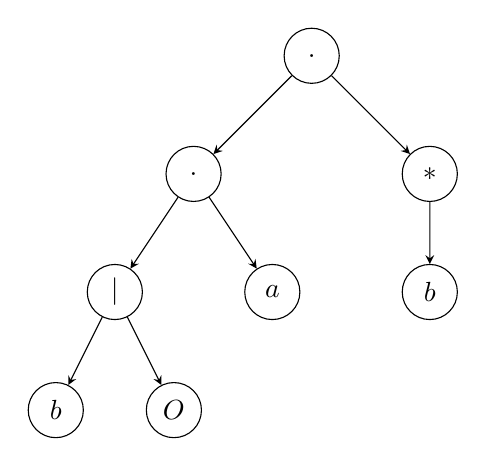
\begin{tikzpicture}
    [level 1/.style={sibling distance=30mm},
    level 2/.style={sibling distance=20mm},
    level 3/.style={sibling distance=15mm},
    nodes={draw,circle,inner sep=0pt, minimum size=7mm},
    ->,>=stealth]
    
    \node {$\rx.$}
    child { node {$\rx.$}  edge from parent
      % [level 2/.style={sibling distance=15mm}]
      child { node {$\rx{|}$}  edge from parent
        % [level 2/.style={sibling distance=15mm}]
        child { node {$\rx{b}$}  edge from parent
          % [level 2/.style={sibling distance=15mm}]
        }
        child { node {$\rx{O}$}  edge from parent
          % [level 2/.style={sibling distance=15mm}]
        }
      }
      child {node {$\rx{a}$} edge from parent}
    }
    child { node {$\rx{*}$}  edge from parent
      % [level 2/.style={sibling distance=15mm}]
      child { node {$\rx{b}$}  edge from parent
        % [level 2/.style={sibling distance=15mm}]
      }
    }
    ;
  \end{tikzpicture}
  \caption{Der Kantorowitsch-Baum für den regulären Ausdruck $\protect\rx{((b|O)a)(b*)}$}
  \label{fig:kantorowitsch-baum}
\end{figure}

Hier handelt es sich \emph{nicht} um den Ableitungsbaum gemäß der
Grammatik aus Abschnitt~\ref{sec:reg-ausdruecke}. Aber die Struktur
des regulären Ausdruckes wird offensichtlich ebenso gut wiedergegeben
und die Darstellung ist sogar noch kompakter.
%
\begin{tutorium}
  \subsubsection*{Kantorowitsch-Bäume}
  Kantorowitsch-Bäume führ ich nicht formal ein. Zur weiteren
  Erläuterung vielleicht auch noch mal einen arithmetischen Ausdruck
  wie $3+(a+b)*(-c)$ umwandeln in

  \begin{center}
    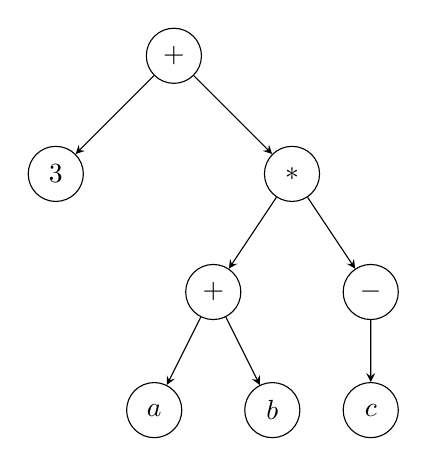
\begin{tikzpicture}
      [level 1/.style={sibling distance=30mm},
      level 2/.style={sibling distance=20mm},
      level 3/.style={sibling distance=15mm},
      nodes={draw,circle,inner sep=0pt, minimum size=7mm},
      ->,>=stealth]
      
      \node {$+$}
      child { node {$3$}  edge from parent  }
      child { node {$*$}  edge from parent
        % [level 2/.style={sibling distance=15mm}]
        child { node {$\rx{+}$}  edge from parent
          % [level 2/.style={sibling distance=15mm}]
          child { node {$a$}  edge from parent
            % [level 2/.style={sibling distance=15mm}]
          }
          child { node {$b$}  edge from parent
            % [level 2/.style={sibling distance=15mm}]
          }
        }
        child {node {$-$} edge from parent
          child { node {$c$}  edge from parent}
        }
      }
      ;
    \end{tikzpicture}
  \end{center}
\end{tutorium}

\begin{tutorium}
  \subsubsection*{Regex-Bäume}
  Das ist natürlich kein feststehender Begriff. Ich benutzt ihn nur, um
  mir nicht den Mund fusselig zu reden.
\end{tutorium}
Solche Bäume wollen wir im folgenden der Einfachheit halber
Regex-Bäume nennen.  Es sei $A$ irgendein Alphabet. Dann ist
ein Baum ein Regex-Baum, wenn gilt:
\begin{itemize}
\item Entweder ist es ein Baum, dessen Wurzel zugleich Blatt ist, und
  das ist mit einem $x\in A$ oder $\rx{O}$ beschriftet,
\item oder es ist ein Baum, dessen Wurzel mit $\rx*$ beschriftet ist
  und die genau einen Nachfolgeknoten hat, der Wurzel eines
  Regex-Baumes ist
\item oder es ist ein Baum, dessen Wurzel mit
  \textcolor{darkblue}{$\cdot$} oder mit $\rx|$ beschriftet ist und
  die genau zwei Nachfolgeknoten hat, die Wurzeln zweier Regex-Bäume
  sind.
\end{itemize}
%
Man beachte, dass linker und rechter Unter-Regex-Baum unterhalb der
Wurzel unterschiedliche Höhe haben können.

Wichtig ist für uns im folgenden, dass erstens größere Bäume "`aus
kleineren zusammengesetzt"' werden, und dass zweitens diese
Zusammensetzung immer eindeutig ist. Außerdem kommt man bijektiv von
regulären Ausdrücken zu Regex-Bäumen und umgekehrt.

Für das weitere definieren wir noch ein oft auftretendes Maß für
Bäume, die sogenannte \mdefine[Höhe eines Baumes]{Höhe}%
\index{Höhe eines Baumes}\index{Baum!Höhe} $h(T)$ eines Baumes
$T$. Das geht so:
\[
h(T) =
\begin{cases}
  0 & \text{ falls die Wurzel Blatt ist }\\
  1+\max_i h(U_i) & \text{ falls die $U_i$ alle Unterbäume von $T$ sind}
\end{cases}
\]
\begin{tutorium}
  \subsubsection*{Höhe von Bäumen}
  Kann man auch definieren als Länge der längsten
  (wiederholungsfreien) Wege von der Wurzel zu irgendwelchen Blättern.

  Eventuell die etwas lasche Formulierung des Falles "`$1+\max_i
  h(U_i)$, falls \dots"' erläutern
\end{tutorium}

Wenn man beweisen möchte, dass eine Aussage für alle regulären
Ausdrücke gilt, dann kann man das dadurch tun, dass man die
entsprechende Aussage für alle Regex-Bäume beweist. Und den Beweis für
alle Regex-Bäume kann man durch vollständige Induktion über ihre Höhe
führen. Bei naiver Herangehensweise tritt aber ein Problem auf: Beim
Schritt zu Bäumen der Höhe $n+1$
darf man nur auf Bäume der Höhe $n$
zurückgreifen. Auftretende Unterbäume können aber alle Höhen $i\leq n$
haben, und man möchte gerne für sie alle die Induktionsvoraussetzung
benutzen. Das darf man auch, wie wir uns in
Kapitel~\ref{k:induktives-vorgehen} klar gemacht haben.

% Das darf man auch! Wir wollen uns zunächst klar machen,
% warum das so ist.

% Dazu sehen wir uns eine einfache Verallgemeinerung vollständiger
% Induktion an. Es sei $\B(n)$ eine Aussage, die von einer Zahl
% $n\in\N_0$ abhängt. Wir wollen beweisen: $\forall n\in \N_0: \B(n)$.
% Dazu definieren wir eine Aussage $\A(n)$ wie folgt: $\forall i\leq n:
% \B(i)$. Wenn wir beweisen können, dass $\forall n\in \N_0: \A(n)$
% gilt, dann sind wir fertig, denn aus $\A(n)$ folgt stets $\B(n)$.

% Wie sieht ein Induktionsbeweis für $\forall n\in \N_0: \A(n)$ aus?

% \begin{description}
% \item[\textcolor{darkred}{Induktionsanfang}:] Es ist zu zeigen, dass
%   $\A(0)$ gilt, also die Aussage $\forall i\leq 0: \B(i)$. Das ist
%   offensichtlich äquivalent zu $\B(0)$. Das ist zu zeigen.
% \item[\textcolor{darkred}{Induktionsvoraussetzung}:] für beliebiges
%   aber festes $n\in\N_0$ gilt: $\A(n)$, also die Aussage $\forall
%   i\leq n:\B(i)$.
% \item[\textcolor{darkred}{Induktionsschluss}:] Es ist zu zeigen, dass
%   auch $\A(n+1)$ gilt, also die Aussage $\forall i\leq n+1:
%   \B(i)$. Diese Aussage ist äquivalent zu $\Bigl(\forall i\leq n:
%   \B(i)\Bigr) \land \B(n+1)$. Wie zeigt man das?
%   \begin{itemize}
%   \item Der erste Teil $\forall i\leq n: \B(i)$ ist trivial, denn das
%     ist ja gerade die Induktionsvoraussetzung.
%   \item Daher bleibt nur zu zeigen: $\B(n+1)$. Zum Beweis dafür kann
%     man aber ebenfalls auf die Induktionsvoraussetzung zurückgreifen,
%     also auf \emph{alle} Aussagen $\B(0)$, $\B(1)$, \dots, $\B(n)$
%     und nicht nur die letzte von ihnen.
%   \end{itemize}
% \end{description}
% %

Das wollen wir nun anwenden, um zu einen Beweis dafür zu skizzieren,
dass es für jeden regulären Ausdruck $R$ eine rechtslineare Grammatik
$G$ gibt mit $\lang{R}=L(G)$.
%
Bei regulären Ausdrücken denkt man nun vorteilhafterweise an
Regex-Bäume und wir machen nun zunächst eine "`normale"' vollständige
Induktion über die Höhe der Regex-Bäume. Im Schema von eben ist also
$\B(n)$ die Aussage:

\begin{quote}
  Für jeden Regex-Baum $R$ der Höhe $n$ gibt es eine rechtslineare
  Grammatik $G$ mit $\lang{R}=L(G)$.
\end{quote}
%
Wir wollen zeigen, dass $\forall n\in\N_0: \B(n)$ gilt.

\begin{description}
\item[\textcolor{darkred}{Induktionsanfang}:] Es ist $\B(0)$ zu
  zeigen. Man muss also rechtslineare Grammatiken angeben, die die
  formalen Sprachen $\{x\}=\lang{x}$ für $x\in A$ und die leere Menge
  $\{\}=\lang{\rx{O}}$ erzeugen. Das ist eine leichte Übung.
\item[\textcolor{darkred}{Induktionsschluss}:] Es ist zu zeigen, dass
  für jedes $n\in\N_0$ aus $\B(n)$ auch $\B(n+1)$ folgt. Dazu sei für
  $n\in\N_0$ die \textcolor{darkred}{Induktionsvoraussetzung}, dass
  für jedes $i\leq n$ $\B(i)$ gilt, dass es also für jeden Regex-Baum
  $R'$ mit einer Höhe $i\leq n$ eine rechtslineare Grammatik $G$ mit
  $\lang{R'}=L(G)$ existiert.

  Sei nun $R$ ein beliebiger Regex-Baum der Höhe $n+1$. Dann gibt es
  drei mögliche Fälle:
  \begin{enumerate}
  \item Die Wurzel von $R$ ist ein $\rx*$-Knoten und hat genau einen
    Unterbaum $R'$ der Höhe $n$.
  \item Die Wurzel von $R$ ist ein $\rx|$-Knoten und hat genau zwei
    Unterbäume $R_1$ und $R_2$. Da $R$ Höhe $n+1$ hat, hat einer der
    beiden Unterbäume Höhe $n$, der andere hat eine Höhe $i\leq n$.
  \item Die Wurzel von $R$ ist ein "`Konkatenations-Knoten"' und hat
    genau zwei Unterbäume $R_1$ und $R_2$. Da $R$ Höhe $n+1$ hat, hat
    einer der beiden Unterbäume Höhe $n$, der andere hat eine Höhe
    $i\leq n$.
  \end{enumerate}
  %
  Der entscheidende Punkt ist nun: In den Fällen 2 und 3 darf man nach
  Induktionsvoraussetzung annehmen, dass für \emph{beide} Unterbäume
  rechtslineare Grammatiken der gewünschten Art existieren.

  In allen drei Fällen kann man dann aus den Grammatiken für den
  Unterbaum \bzw die Unterbäume die Grammatik für den Regex-Baum, also
  regulären Ausdruck, $R$ konstruieren. Das wollen wir hier nicht
  in allen Details durchführen und beschränken uns auf den einfachsten
  Fall, nämlich Fall 2: Seien also $G_1=(N_1,A,S_1,P_1)$ und
  $G_2=(N_2,A,S_2,P_2)$ Typ-3-Grammatiken, die $L(G_1)=\lang{R_1}$
  \bzw $L(G_2)=\lang{R_2}$ erzeugen. Ohne Beschränkung der
  Allgemeinheit nehmen wir an, dass $N_1\cap N_2=\{\}$ ist. Wir
  wählen ein "`neues"' Nichtterminalsymbol $S\notin N_1\cup N_2$ Damit
  können wir eine Typ-3-Grammatik $G$ mit $L(G)=\lang{R_1\rx| R_2}$
  ganz leicht hinschreiben:
  \[
  G = (\{S\}\cup N_1\cup N_2, A, S, \{ S-> S_1\mid S_2\} \cup P_1\cup P_2)
  \]
  Als erstes muss man sich klar machen, dass auch die Grammatik
  rechtslinear ist. Tun Sie das; es ist nicht schwer. 

  Etwas Arbeit würde es machen, zu beweisen, dass $L(G)=L(G_1)\cup
  L(G_2)$ ist. Das wollen wir uns an dieser Stellen sparen.
  Sie können das aber ruhig selbst einmal versuchen. 

  Und für die anderen beiden Fälle können Sie das auch einmal
  versuchen, geeignete (rechtslineare!) Grammatiken zu konstruieren,
  oder einfach glauben, dass es geht.
\end{description}

\noindent
Um zu einer manchmal sogenannten \mdefine[strukturelle
Induktion]{strukturellen Induktion}\index{strukturelle Induktion}%
\index{Induktion!strukturelle} zu kommen, muss man nun nur noch
das Korsett der vollständigen Induktion über die Höhe der Bäume
"`vergessen"'. Was bleibt ist folgende prinzipielle Situation:
\begin{enumerate}
\item Man beschäfigt sich mit irgendwelchen "`Gebilden"' (eben waren
  das reguläre Ausdrücke \bzw Bäume). Dabei gibt es kleinste
  "`atomare"' oder "`elementare"' Gebilde (eben waren das die
  regulären Ausdrücke $x$ für $x\in A$ und $\rx{O}$) und eine oder
  mehrere Konstruktionsvorschriften, nach denen man aus kleineren
  Gebilden größere zusammensetzen kann (eben waren das $\rx*$, $\rx|$
  und Konkatenation).
\item Man möchte beweisen, dass alle Gebilde eine gewisse Eigenschaft
  haben. Dazu macht man dann eine strukturelle Induktion:
  \begin{itemize}
  \item Im Induktionsanfang zeigt man zunächst für \emph{alle}
    "`atomaren"' Gebilde, dass sie eine gewünschte Eigenschaft haben
    und
  \item im Induktionsschritt zeigt man, wie sich bei einem "`großen"'
    Gebilde die Eigenschaft daraus folgt, dass schon alle Untergebilde
    die Eigenschaft haben, gleich nach welcher Konstruktionsvorschrift
    das große Gebilde gebaut ist.
  \end{itemize}
\end{enumerate}

%-----------------------------------------------------------------------
\section{Ausblick}

Beweise für die Behauptungen aus Satz~\ref{thm:reg-exp<->dfa<->typ-3}
werden Sie vielleicht in der Vorlesung "`Theoretische Grundlagen der
Informatik"' oder in "`Formale Systeme"' sehen. Insbesondere ist es
dafür nützlich, sich mit nichtdeterministischen endlichen Automaten zu
beschäftigen, auf die wir am Ende von Einheit~\ref{k:endl-auto} schon
hingewiesen haben.

Sie werden sehen, dass reguläre Ausdrücke bei der Verarbeitung von
Textdateien des Öfteren nützlich sind. Dabei kommen zu dem, was wir in
Abschnitt~\ref{sec:reg-ausdruecke} definiert haben, zum einen noch
bequeme Abkürzungen hinzu, denn wer will schon \zB
\[
\rx{a|b|c|d|e|f|g|h|i|j|k|l|m|n|o|p|q|r|s|t|u|v|w|x|y|z}
\]
schreiben müssen als regulären Ausdruck für einen einzelnen
Kleinbuchstaben. Zum anderen gibt es aber auch noch Erweiterungen, die
dazu führen, dass die resultierenden \emph{regular expressions}
mächtiger sind als reguläre Ausdrücke. Wer sich dafür (jetzt schon)
genauer interessiert, dem sei das Buch von
\textcite{Friedl_2006_MRE_bk} empfohlen.

% -----------------------------------------------------------------------
% Literatur
%  if something has been cited in this unit:
\printunitbibliography

\cleardoublepage

%-----------------------------------------------------------------------
%%%
%%% Local Variables:
%%% fill-column: 70
%%% mode: latex
%%% TeX-master: "../k-19-reg-ausdruecke/skript.tex"
%%% TeX-command-default: "XPDFLaTeX"
%%% End:
